\documentclass[twoside,english,a4paper,12pt]{plantilla/twcam-tfm-doc}

% Editar el título
\title{Este es un muy largo título usado de prueba para ver cómo se formatea en varias líneas en la portada}

% Si es una alumna se debe usar
% \authorlabel{Autora}
\authorlabel{Autor}
% Editar el nombre
\author{Mi nombre}


% Si hay varios tutores:
% \tutorlabel{Tutores}
% \tutor{Nombre del tutor 1 \\[2mm] Nombre del turor2}
% Si el tutor es masculino:
% \tutorlabel{Tutor}
\tutorlabel{Tutora}
% Editar
\tutor{El nombre de la tutora}

% Editar: Poner mes y año de la convocatoria de lectura del TFM
\convocatoria{Julio 2019}

\usepackage[xindy,style=altlist,numberline,savewrites=true,acronym]{glossaries}
\usepackage[spanish]{babel}
\usepackage[numbers]{natbib}
\usepackage{doi}
\usepackage{eurosym}
\usepackage{longtable}
\usepackage{array}
\usepackage{rotating}
\usepackage{nameref}
\usepackage{pdfpages}

\makeglossaries
\loadglsentries{tex/acronimos-y-terminos.tex}

\makeatletter
\newcommand*{\mySetNameref}{\def\@currentlabelname}

\newcommand\YAMLcolonstyle{\color{red}\mdseries}
\newcommand\YAMLkeystyle{\color{black}\bfseries}
\newcommand\YAMLvaluestyle{\color{blue}\mdseries}
\definecolor{mygray}{rgb}{0.5,0.5,0.5}

\newcommand\language@yaml{yaml}

\expandafter\expandafter\expandafter\lstdefinelanguage
\expandafter{\language@yaml}
{
  keywords={true,false,null,y,n},
  keywordstyle=\color{darkgray}\bfseries,
  basicstyle=\YAMLkeystyle,                                 % assuming a key comes first
  sensitive=false,
  numbers=none,                    % where to put the line-numbers; possible values are (none, left, right)
  numbersep=5pt,                   % how far the line-numbers are from the code
  numberstyle=\tiny\color{mygray}, % the style that is used for the line-numbers
  comment=[l]{\#},
  morecomment=[s]{/*}{*/},
  commentstyle=\color{purple}\ttfamily,
  stringstyle=\YAMLvaluestyle\ttfamily,
  moredelim=[l][\color{orange}]{\&},
  moredelim=[l][\color{magenta}]{*},
  moredelim=**[il][\YAMLcolonstyle{:}\YAMLvaluestyle]{:},   % switch to value style at :
  morestring=[b]',
  morestring=[b]",
  literate =    {---}{{\ProcessThreeDashes}}3
                {>}{{\textcolor{red}\textgreater}}1     
                {|}{{\textcolor{red}\textbar}}1 
                {\ -\ }{{\mdseries\ -\ }}3,
}

% switch to key style at EOL
\lst@AddToHook{EveryLine}{\ifx\lst@language\language@yaml\YAMLkeystyle\fi}
\makeatother

\begin{document}

\renewcommand{\listtablename}{Índice de tablas}
\renewcommand{\tablename}{Tabla}

% NO QUITAR ESTOS ELEMENTOS
\portada
\cleardoublepage
\contraportada
\cleardoublepage
\declaracion
\cleardoublepage


% Editar: Resumen en Español (obligatorio)
\begin{resumen}
  Este es el resumen del TFM. Debe ser corto (máximo media página) y cubrir los aspectos principales del TFM.
\end{resumen}
\cleardoublepage

% Editar: Resumen en Inglés
\begin{abstract}
  This is the abstract of the TFM. It must be short and cover the main aspects of the TFM.
\end{abstract}
\cleardoublepage

% Editar: Resumen en Valenciano
\begin{resum}
  Aquest és el resum del TFM. Ha de ser curt (màxim mitja pàgina) i cobrir els aspectes principals del TFM.
\end{resum}
\cleardoublepage


% Editar: Agradecimientos (opcional)
\begin{agradecimientos}
  En primer lugar quiero agradecer a...

  En segundo lugar...
\end{agradecimientos}
\cleardoublepage

\tableofcontents

\listoffigures

\cleardoublepage

\listoftables

\cleardoublepage

\lstlistoflistings

\cleardoublepage

\pagestyle{twcam}
\justify

% Las figuras se buscan en el directorio figs

% Cada capítulo está en su propio fichero tex. Ver el directorio tex.

% La bibliografía está dentro del directorio bib
\chapter{Introducción}
% Contenidos del capítulo.
% Las secciones presentadas son orientativas y no representan
% necesariamente la organización que debe tener este capítulo.



\section{Introducción}

\section{Motivación}

\section{Objetivos}

\section{Organización de la memoria}



\chapter{Estado del arte}
% Contenidos del capítulo.
% Las secciones presentadas son orientativas y no representan
% necesariamente la organización que debe tener este capítulo.

\section{Análisis de aplicaciones similares}
% Qué aplicaciones similares hay y en qué se diferencia de ellas la propuesta

\section{Tecnologías}
% Análisis crítico de las tecnologías y sistemas de despliegue posibles y por qué se han seleccionado unas concretas.



\chapter{Requisitos, especificaciones, coste, riesgos, viabilidad}
% Contenidos del capítulo
%Las secciones presentadas son orientativas y no representan necesariamente la organización que debe tener este capítulo.

\section{Requisitos}
Requisitos funcionales y no funcionales del proyecto.

Se debe optar por formular los requisitos de forma que se pueda
conocer si se han alcanzado o no a la finalización del proyecto. Por
ejemplo, es difícil valorar si el siguiente requisito funcional se
alcanza o no: \textit{El sistema debe retornar una respuesta en un tiempo
razonable cuando tenga muchos usuarios concurrentes}. ¿Cuánto es un
tiempo razonable?, ¿cuantos son muchos usuarios?. Sin embargo, si se
formula de este otro modo: \textit{El sistema debe retornar una
respuesta en menos de un segundo cuando tenga 200 usuarios
concurrentes}, es fácil comprobar si se ha alcanzado ejecutando un
plan de pruebas, por ejemplo con JMeter.

\section{Especificaciones}
Especificación del proyecto a partir de los requisitos.

\section{Planificación y estimación de costes}
Describir el tipo de metodología de desarrollo que se va a utilizar
(cascada, ágil, etc).

Tareas a realizar, estimación de la duración de las tareas, y
distribución temporal (por ejemplo con un diagrama de Gantt).

Costes de personal (teniendo en cuenta los costes de seguridad
social), de hardware (imputando solo la duración del proyecto y teniendo
en cuenta que los equipos se amortizan en 3 o 4 años) y/o de software.
Además, hay que añadir costes indirectos.

\section{Riesgos}

Identificación de los riesgos que pueden aparecer durante el
desarrollo del proyecto, su probabilidad de ocurrencia, su impacto en
el proyecto y las medidas que se podrían adoptar para mitigarlos.

\section{Viabilidad}
En este apartado, dependiendo de la naturaleza del proyecto, se
debería analizar la viabilidad técnica y la viabilidad económica. Para
la viabilidad técnica hay que analizar si los recursos
necesarios (herramientas, conocimientos, experiencia, etc)  para llevar
a cabo el proyecto permiten realizarlo en el tiempo previsto.
En cuanto a la viabilidad económica hay que evaluar si el proyecto
será rentable cuando esté operativo.


\chapter{Análisis}
% Contenidos del capítulo.

En este capítulo se analiza \textbf{qué} debe hacer la aplicación.

Los contenidos que se presentan a continuación pueden variar y se deben adaptar a la naturaleza de la aplicación.

Se debe analizar la aplicación e identificar los casos de uso, modelado de datos, el tipo de despliegue de la aplicación, etc.


\chapter{Diseño}
% Contenidos del capítulo.

El capítulo de diseño presenta \textbf{cómo} se va a abordar desde el punto de vista técnico
lo que se ha presentado en la fase de análisis.

Los contenidos  presentados son orientativas y se deberán adaptar a la
naturaleza del trabajo realizado.

Diagramas de clases, de secuencia, de despliegue, diseño de pantallas,
diseño de la base de datos, etc.

\chapter{Implementación y pruebas}
% Contenidos del capítulo.
Las secciones presentadas son orientativas y no representan
necesariamente la organización que debe tener este capítulo.
\section{Implementación}
Presentar cómo se ha organizado el desarrollo de los proyectos
(capturas del IDE), trozos de código relevantes, cómo han quedado
implementadas las interfaces gráficas de usuario, etc.
\section{Pruebas unitarias}
Descripción de las pruebas que se han llevado a cabo para comprobar que el código
desarrollado es correcto (JUnit, etc).
\section{Pruebas funcionales}
Descripción de las pruebas que se han llevado a cabo para comprobar que los casos de uso
identificados funcionan correctamente.
\section{Pruebas de rendimiento}
Descripción de las pruebas de estrés realizadas para comprobar los tiempos de
respuesta de la aplicación (según figuren en los requisitos).
\section{Pruebas de usabilidad}
Descripción de las pruebas que se han llevado a cabo con usuarios para determinar el
nivel de usabilidad de la aplicación (que se hayan recogido en los requisitos).
\section{Pruebas de seguridad}
Descripción de las pruebas realizadas para comprobar que se cumplen las
restricciones de autenticación y de autorización que se han descrito
en los requisitos.
\chapter{Conclusiones}
% Contenidos del capítulo.
% Las secciones presentadas son orientativas y no representan
% necesariamente la organización que debe tener este capítulo.

\section{Revisión de costes}

\section{Conclusiones}

\section{Trabajo futuro}

\addcontentsline{toc}{chapter}{Acrónimos}
\printglossary[type=\acronymtype, title=Acrónimos, toctitle=Acrónimos]
\mySetNameref{Acrónimos}%
\label{ch:acronimos}


\addcontentsline{toc}{chapter}{Glosario}
\printglossary[type=main, title=Glosario, toctitle=Glosario]
\mySetNameref{Glosario}%
\label{ch:glo}

\pagestyle{appendix}

\appendix
\chapter{Apéndice ejemplo}
\section{Ejemplos del lenguaje de marcado Latex}

Ejemplos de citas: el libro \textit{The \LaTeX\ Companion}
\cite{latexcompanion}, un paper de Einstein \cite{einstein}, dos informes técnicos de relevancia \cite{NIST:Cloud-2011,OWASP:Top10-2017} y la página de la ETSE sobre TFMs \cite{ETSE:online}\footnote{Esto está tomado de
\url{https://www.overleaf.com/learn/latex/Bibliography_management_with_bibtex}}.

Ejemplo de uso de acrónimos en sigular \gls{tfm} y en plural \glspl{tfm}.

Ejemplo de uso de un término de glosario como es \gls{backend}.


  \textbf{Texto} en el párrafo 1.

  \textit{Texto} en el párrafo 2.

  \texttt{Texto} en el párrafo 3.


  \begin{itemize}
  \item Consideración 1
  \item Consideración 2
  \end{itemize}

  % Espacio vertical
  \vspace{0.5cm}

  \begin{enumerate}
  \item Punto 1
  \item Punto 2
  \end{enumerate}

A continuación se muestra una ecuación:

  \[ \int_{0}^{1}\frac{1}{x^2+1} dx \]

  Podemos incluir imágenes en formato: png, pdf o jpg.

  En la Figura~\ref{fig:diagrama} se muestra un diagrama realizado con \href{yed}{https://www.yworks.com/products/yed}:

  \begin{figure}[!htb]
    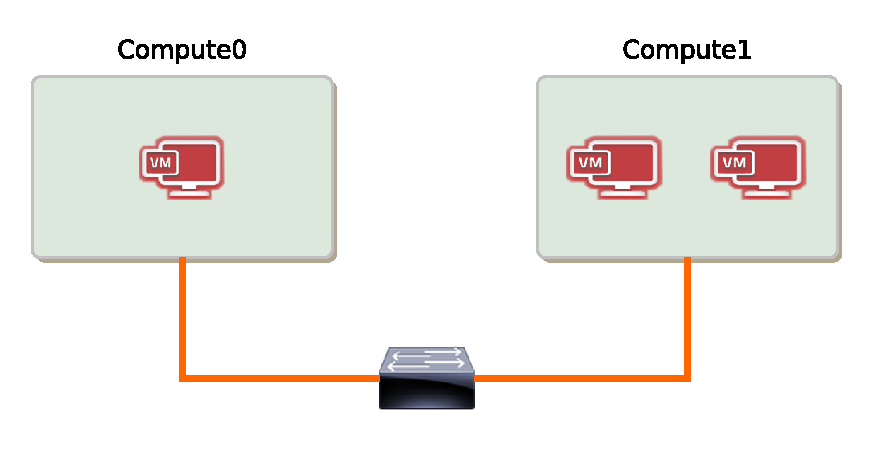
\includegraphics[width=0.8\textwidth]{diagrama.pdf}
    \caption{Esta es una figura que latex decide donde colocar (floating) en el documento.}
    \label{fig:diagrama}
    \end{figure}

    Latex decide dónde poner los elementos flotantes (figure o table)
    aunque usemos \verb#!htb# que significa: intenta poner el elemento
    aquí (h:here), al inicio de la página (t: top) o al final de la
    página (b: bottom). Sin embargo, a veces quedan demasiado lejos de
    donde son citados. Si esto ocurre puedes usar la orden
    \verb#\cleardoublepage# para que vacíe el buffer de elementos flotantes.

  \begin{tabular}{cc}
    Imagen 1 & Imagen 2 \\[2mm]
    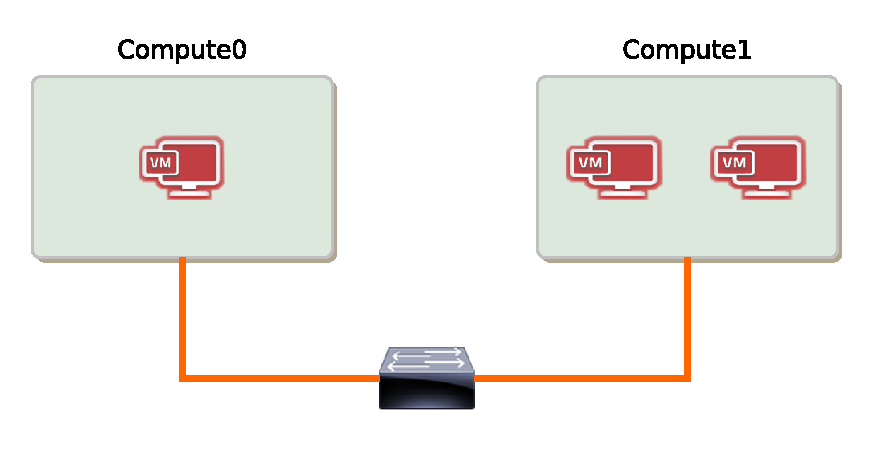
\includegraphics[width=0.4\textwidth]{diagrama.pdf} &  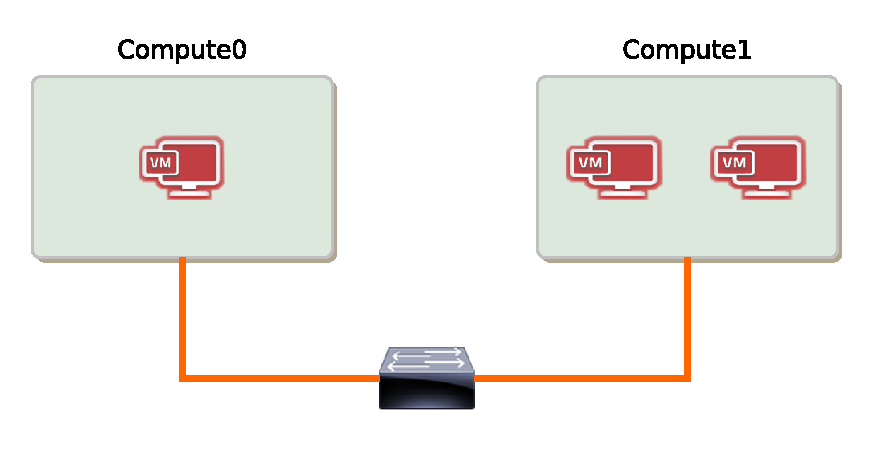
\includegraphics[width=0.4\textwidth]{diagrama.pdf}
  \end{tabular}

  La Tabla \ref{tbl:ejemplo} muestra un ejemplo.

\begin{table}[h!tb]
  \caption{Ejemplo de tabla \label{tbl:ejemplo}}
  \begin{tabular}{|l|c|}
    \hline
    Columna 1 & Columna 2 \\ \hline
    1 & 2 \\ \hline
  \end{tabular}
\end{table}


  \vspace*{1cm}
  Mientras que la Tabla \ref{tbl:centrada} muestra la misma tabla centrada. 

  \begin{table}[h!tb]
  \caption{Ejemplo de tabla centrada \label{tbl:centrada}}
  \begin{center}
    \begin{tabular}{|l|c|}
      \hline
      Columna 1 & Columna 2 \\ \hline
      1 & 2 \\ \hline
    \end{tabular}
  \end{center}
  
\end{table}

  Para generar el fichero PDF podemos usar los comandos que muestra el Listao \ref{lst:cmds}.

  \begin{lstlisting}[language=bash,caption={Comandos para generar PDF con pdflatex},label={lst:cmds}]
    pdflatex ejemplo-memoria.tex
    bibtex ejemplo-memoria
    pdflatex ejemplo-memoria.tex
\end{lstlisting}

  También se puede usar \texttt{latexmk} que automáticamente regenera la bibliografía, tal y como muestra el Listado \ref{lst:latexmk}.

  \begin{lstlisting}[language=bash,caption={Comandos para generar PDF con latexmk},label={lst:latexmk}]
    latexmk -pdf ejemplo-memoria.tex
\end{lstlisting}


\chapter{Apéndice incluyendo ficheros {\tt PDF}}
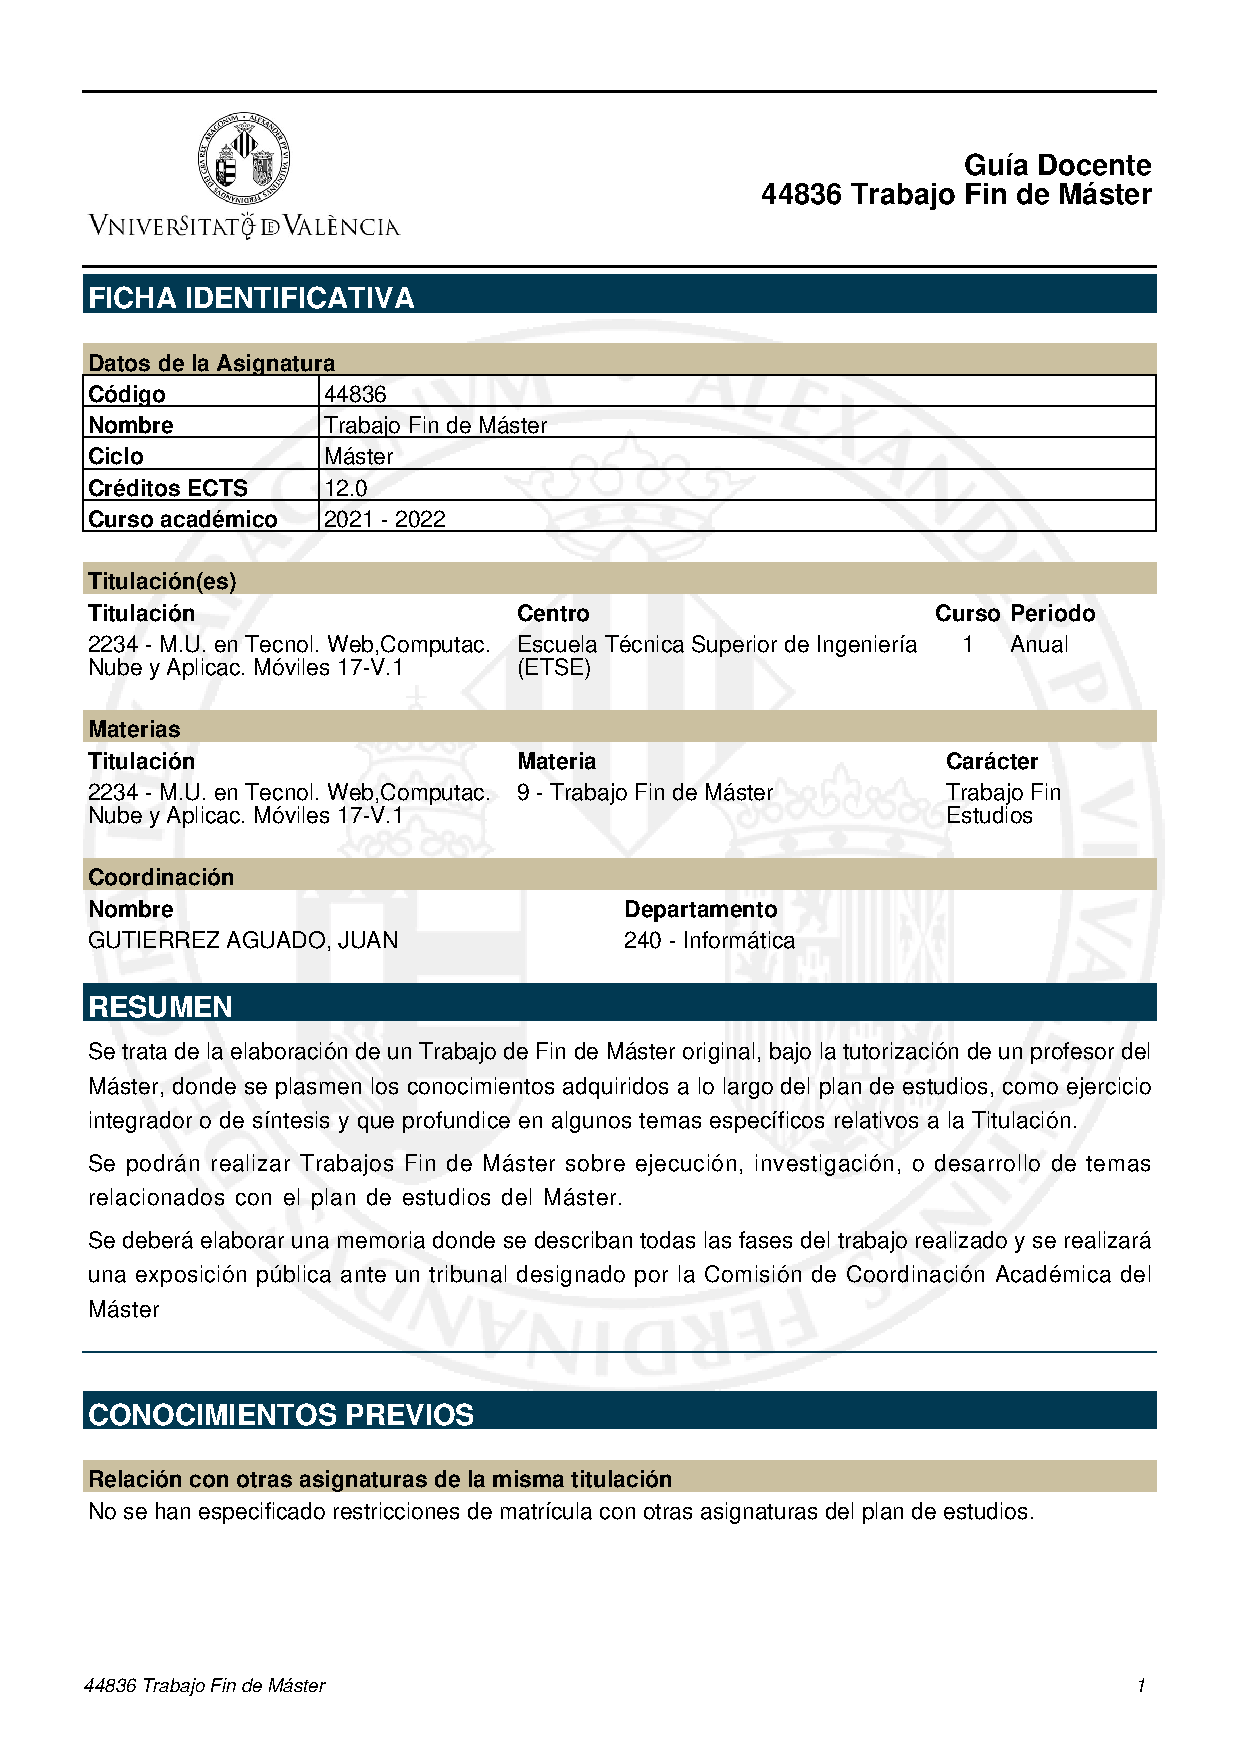
\includepdf[pages={1-last},
nup=1x1,frame=true,landscape=false, offset=0 0,deltax=5,deltay=10, scale=.8,pagecommand={\pagestyle{headings}}]
{../docs/guia-tfm.pdf}

\chapter{Apéndice incluyendo listados de ficheros}
\section{Ficheros de despliegue}

\lstinputlisting[language=yaml,caption={Ejemplo de docker-compose}]{docs/docker-compose.yaml}

\section{Ficheros de scripts}

\lstinputlisting[language=bash,caption={Script para generación de PDF desde \LaTeX{}}]{docs/latex2pdf.sh}


\addcontentsline{toc}{chapter}{Bibliografía}
\bibliographystyle{unsrtnat}
\bibliography{bib/bibliografia}




\end{document}

%%% Local Variables:
%%% mode: latex
%%% TeX-master: t
%%% End:
